
% Default to the notebook output style

    


% Inherit from the specified cell style.




    
\documentclass[11pt]{article}

    
    
    \usepackage[T1]{fontenc}
    % Nicer default font (+ math font) than Computer Modern for most use cases
    \usepackage{mathpazo}

    % Basic figure setup, for now with no caption control since it's done
    % automatically by Pandoc (which extracts ![](path) syntax from Markdown).
    \usepackage{graphicx}
    % We will generate all images so they have a width \maxwidth. This means
    % that they will get their normal width if they fit onto the page, but
    % are scaled down if they would overflow the margins.
    \makeatletter
    \def\maxwidth{\ifdim\Gin@nat@width>\linewidth\linewidth
    \else\Gin@nat@width\fi}
    \makeatother
    \let\Oldincludegraphics\includegraphics
    % Set max figure width to be 80% of text width, for now hardcoded.
    \renewcommand{\includegraphics}[1]{\Oldincludegraphics[width=.8\maxwidth]{#1}}
    % Ensure that by default, figures have no caption (until we provide a
    % proper Figure object with a Caption API and a way to capture that
    % in the conversion process - todo).
    \usepackage{caption}
    \DeclareCaptionLabelFormat{nolabel}{}
    \captionsetup{labelformat=nolabel}

    \usepackage{adjustbox} % Used to constrain images to a maximum size 
    \usepackage{xcolor} % Allow colors to be defined
    \usepackage{enumerate} % Needed for markdown enumerations to work
    \usepackage{geometry} % Used to adjust the document margins
    \usepackage{amsmath} % Equations
    \usepackage{amssymb} % Equations
    \usepackage{textcomp} % defines textquotesingle
    % Hack from http://tex.stackexchange.com/a/47451/13684:
    \AtBeginDocument{%
        \def\PYZsq{\textquotesingle}% Upright quotes in Pygmentized code
    }
    \usepackage{upquote} % Upright quotes for verbatim code
    \usepackage{eurosym} % defines \euro
    \usepackage[mathletters]{ucs} % Extended unicode (utf-8) support
    \usepackage[utf8x]{inputenc} % Allow utf-8 characters in the tex document
    \usepackage{fancyvrb} % verbatim replacement that allows latex
    \usepackage{grffile} % extends the file name processing of package graphics 
                         % to support a larger range 
    % The hyperref package gives us a pdf with properly built
    % internal navigation ('pdf bookmarks' for the table of contents,
    % internal cross-reference links, web links for URLs, etc.)
    \usepackage{hyperref}
    \usepackage{longtable} % longtable support required by pandoc >1.10
    \usepackage{booktabs}  % table support for pandoc > 1.12.2
    \usepackage[inline]{enumitem} % IRkernel/repr support (it uses the enumerate* environment)
    \usepackage[normalem]{ulem} % ulem is needed to support strikethroughs (\sout)
                                % normalem makes italics be italics, not underlines
    

    
    
    % Colors for the hyperref package
    \definecolor{urlcolor}{rgb}{0,.145,.698}
    \definecolor{linkcolor}{rgb}{.71,0.21,0.01}
    \definecolor{citecolor}{rgb}{.12,.54,.11}

    % ANSI colors
    \definecolor{ansi-black}{HTML}{3E424D}
    \definecolor{ansi-black-intense}{HTML}{282C36}
    \definecolor{ansi-red}{HTML}{E75C58}
    \definecolor{ansi-red-intense}{HTML}{B22B31}
    \definecolor{ansi-green}{HTML}{00A250}
    \definecolor{ansi-green-intense}{HTML}{007427}
    \definecolor{ansi-yellow}{HTML}{DDB62B}
    \definecolor{ansi-yellow-intense}{HTML}{B27D12}
    \definecolor{ansi-blue}{HTML}{208FFB}
    \definecolor{ansi-blue-intense}{HTML}{0065CA}
    \definecolor{ansi-magenta}{HTML}{D160C4}
    \definecolor{ansi-magenta-intense}{HTML}{A03196}
    \definecolor{ansi-cyan}{HTML}{60C6C8}
    \definecolor{ansi-cyan-intense}{HTML}{258F8F}
    \definecolor{ansi-white}{HTML}{C5C1B4}
    \definecolor{ansi-white-intense}{HTML}{A1A6B2}

    % commands and environments needed by pandoc snippets
    % extracted from the output of `pandoc -s`
    \providecommand{\tightlist}{%
      \setlength{\itemsep}{0pt}\setlength{\parskip}{0pt}}
    \DefineVerbatimEnvironment{Highlighting}{Verbatim}{commandchars=\\\{\}}
    % Add ',fontsize=\small' for more characters per line
    \newenvironment{Shaded}{}{}
    \newcommand{\KeywordTok}[1]{\textcolor[rgb]{0.00,0.44,0.13}{\textbf{{#1}}}}
    \newcommand{\DataTypeTok}[1]{\textcolor[rgb]{0.56,0.13,0.00}{{#1}}}
    \newcommand{\DecValTok}[1]{\textcolor[rgb]{0.25,0.63,0.44}{{#1}}}
    \newcommand{\BaseNTok}[1]{\textcolor[rgb]{0.25,0.63,0.44}{{#1}}}
    \newcommand{\FloatTok}[1]{\textcolor[rgb]{0.25,0.63,0.44}{{#1}}}
    \newcommand{\CharTok}[1]{\textcolor[rgb]{0.25,0.44,0.63}{{#1}}}
    \newcommand{\StringTok}[1]{\textcolor[rgb]{0.25,0.44,0.63}{{#1}}}
    \newcommand{\CommentTok}[1]{\textcolor[rgb]{0.38,0.63,0.69}{\textit{{#1}}}}
    \newcommand{\OtherTok}[1]{\textcolor[rgb]{0.00,0.44,0.13}{{#1}}}
    \newcommand{\AlertTok}[1]{\textcolor[rgb]{1.00,0.00,0.00}{\textbf{{#1}}}}
    \newcommand{\FunctionTok}[1]{\textcolor[rgb]{0.02,0.16,0.49}{{#1}}}
    \newcommand{\RegionMarkerTok}[1]{{#1}}
    \newcommand{\ErrorTok}[1]{\textcolor[rgb]{1.00,0.00,0.00}{\textbf{{#1}}}}
    \newcommand{\NormalTok}[1]{{#1}}
    
    % Additional commands for more recent versions of Pandoc
    \newcommand{\ConstantTok}[1]{\textcolor[rgb]{0.53,0.00,0.00}{{#1}}}
    \newcommand{\SpecialCharTok}[1]{\textcolor[rgb]{0.25,0.44,0.63}{{#1}}}
    \newcommand{\VerbatimStringTok}[1]{\textcolor[rgb]{0.25,0.44,0.63}{{#1}}}
    \newcommand{\SpecialStringTok}[1]{\textcolor[rgb]{0.73,0.40,0.53}{{#1}}}
    \newcommand{\ImportTok}[1]{{#1}}
    \newcommand{\DocumentationTok}[1]{\textcolor[rgb]{0.73,0.13,0.13}{\textit{{#1}}}}
    \newcommand{\AnnotationTok}[1]{\textcolor[rgb]{0.38,0.63,0.69}{\textbf{\textit{{#1}}}}}
    \newcommand{\CommentVarTok}[1]{\textcolor[rgb]{0.38,0.63,0.69}{\textbf{\textit{{#1}}}}}
    \newcommand{\VariableTok}[1]{\textcolor[rgb]{0.10,0.09,0.49}{{#1}}}
    \newcommand{\ControlFlowTok}[1]{\textcolor[rgb]{0.00,0.44,0.13}{\textbf{{#1}}}}
    \newcommand{\OperatorTok}[1]{\textcolor[rgb]{0.40,0.40,0.40}{{#1}}}
    \newcommand{\BuiltInTok}[1]{{#1}}
    \newcommand{\ExtensionTok}[1]{{#1}}
    \newcommand{\PreprocessorTok}[1]{\textcolor[rgb]{0.74,0.48,0.00}{{#1}}}
    \newcommand{\AttributeTok}[1]{\textcolor[rgb]{0.49,0.56,0.16}{{#1}}}
    \newcommand{\InformationTok}[1]{\textcolor[rgb]{0.38,0.63,0.69}{\textbf{\textit{{#1}}}}}
    \newcommand{\WarningTok}[1]{\textcolor[rgb]{0.38,0.63,0.69}{\textbf{\textit{{#1}}}}}
    
    
    % Define a nice break command that doesn't care if a line doesn't already
    % exist.
    \def\br{\hspace*{\fill} \\* }
    % Math Jax compatability definitions
    \def\gt{>}
    \def\lt{<}
    % Document parameters
    \title{aps-redes-neurais}
    
    
    

    % Pygments definitions
    
\makeatletter
\def\PY@reset{\let\PY@it=\relax \let\PY@bf=\relax%
    \let\PY@ul=\relax \let\PY@tc=\relax%
    \let\PY@bc=\relax \let\PY@ff=\relax}
\def\PY@tok#1{\csname PY@tok@#1\endcsname}
\def\PY@toks#1+{\ifx\relax#1\empty\else%
    \PY@tok{#1}\expandafter\PY@toks\fi}
\def\PY@do#1{\PY@bc{\PY@tc{\PY@ul{%
    \PY@it{\PY@bf{\PY@ff{#1}}}}}}}
\def\PY#1#2{\PY@reset\PY@toks#1+\relax+\PY@do{#2}}

\expandafter\def\csname PY@tok@w\endcsname{\def\PY@tc##1{\textcolor[rgb]{0.73,0.73,0.73}{##1}}}
\expandafter\def\csname PY@tok@c\endcsname{\let\PY@it=\textit\def\PY@tc##1{\textcolor[rgb]{0.25,0.50,0.50}{##1}}}
\expandafter\def\csname PY@tok@cp\endcsname{\def\PY@tc##1{\textcolor[rgb]{0.74,0.48,0.00}{##1}}}
\expandafter\def\csname PY@tok@k\endcsname{\let\PY@bf=\textbf\def\PY@tc##1{\textcolor[rgb]{0.00,0.50,0.00}{##1}}}
\expandafter\def\csname PY@tok@kp\endcsname{\def\PY@tc##1{\textcolor[rgb]{0.00,0.50,0.00}{##1}}}
\expandafter\def\csname PY@tok@kt\endcsname{\def\PY@tc##1{\textcolor[rgb]{0.69,0.00,0.25}{##1}}}
\expandafter\def\csname PY@tok@o\endcsname{\def\PY@tc##1{\textcolor[rgb]{0.40,0.40,0.40}{##1}}}
\expandafter\def\csname PY@tok@ow\endcsname{\let\PY@bf=\textbf\def\PY@tc##1{\textcolor[rgb]{0.67,0.13,1.00}{##1}}}
\expandafter\def\csname PY@tok@nb\endcsname{\def\PY@tc##1{\textcolor[rgb]{0.00,0.50,0.00}{##1}}}
\expandafter\def\csname PY@tok@nf\endcsname{\def\PY@tc##1{\textcolor[rgb]{0.00,0.00,1.00}{##1}}}
\expandafter\def\csname PY@tok@nc\endcsname{\let\PY@bf=\textbf\def\PY@tc##1{\textcolor[rgb]{0.00,0.00,1.00}{##1}}}
\expandafter\def\csname PY@tok@nn\endcsname{\let\PY@bf=\textbf\def\PY@tc##1{\textcolor[rgb]{0.00,0.00,1.00}{##1}}}
\expandafter\def\csname PY@tok@ne\endcsname{\let\PY@bf=\textbf\def\PY@tc##1{\textcolor[rgb]{0.82,0.25,0.23}{##1}}}
\expandafter\def\csname PY@tok@nv\endcsname{\def\PY@tc##1{\textcolor[rgb]{0.10,0.09,0.49}{##1}}}
\expandafter\def\csname PY@tok@no\endcsname{\def\PY@tc##1{\textcolor[rgb]{0.53,0.00,0.00}{##1}}}
\expandafter\def\csname PY@tok@nl\endcsname{\def\PY@tc##1{\textcolor[rgb]{0.63,0.63,0.00}{##1}}}
\expandafter\def\csname PY@tok@ni\endcsname{\let\PY@bf=\textbf\def\PY@tc##1{\textcolor[rgb]{0.60,0.60,0.60}{##1}}}
\expandafter\def\csname PY@tok@na\endcsname{\def\PY@tc##1{\textcolor[rgb]{0.49,0.56,0.16}{##1}}}
\expandafter\def\csname PY@tok@nt\endcsname{\let\PY@bf=\textbf\def\PY@tc##1{\textcolor[rgb]{0.00,0.50,0.00}{##1}}}
\expandafter\def\csname PY@tok@nd\endcsname{\def\PY@tc##1{\textcolor[rgb]{0.67,0.13,1.00}{##1}}}
\expandafter\def\csname PY@tok@s\endcsname{\def\PY@tc##1{\textcolor[rgb]{0.73,0.13,0.13}{##1}}}
\expandafter\def\csname PY@tok@sd\endcsname{\let\PY@it=\textit\def\PY@tc##1{\textcolor[rgb]{0.73,0.13,0.13}{##1}}}
\expandafter\def\csname PY@tok@si\endcsname{\let\PY@bf=\textbf\def\PY@tc##1{\textcolor[rgb]{0.73,0.40,0.53}{##1}}}
\expandafter\def\csname PY@tok@se\endcsname{\let\PY@bf=\textbf\def\PY@tc##1{\textcolor[rgb]{0.73,0.40,0.13}{##1}}}
\expandafter\def\csname PY@tok@sr\endcsname{\def\PY@tc##1{\textcolor[rgb]{0.73,0.40,0.53}{##1}}}
\expandafter\def\csname PY@tok@ss\endcsname{\def\PY@tc##1{\textcolor[rgb]{0.10,0.09,0.49}{##1}}}
\expandafter\def\csname PY@tok@sx\endcsname{\def\PY@tc##1{\textcolor[rgb]{0.00,0.50,0.00}{##1}}}
\expandafter\def\csname PY@tok@m\endcsname{\def\PY@tc##1{\textcolor[rgb]{0.40,0.40,0.40}{##1}}}
\expandafter\def\csname PY@tok@gh\endcsname{\let\PY@bf=\textbf\def\PY@tc##1{\textcolor[rgb]{0.00,0.00,0.50}{##1}}}
\expandafter\def\csname PY@tok@gu\endcsname{\let\PY@bf=\textbf\def\PY@tc##1{\textcolor[rgb]{0.50,0.00,0.50}{##1}}}
\expandafter\def\csname PY@tok@gd\endcsname{\def\PY@tc##1{\textcolor[rgb]{0.63,0.00,0.00}{##1}}}
\expandafter\def\csname PY@tok@gi\endcsname{\def\PY@tc##1{\textcolor[rgb]{0.00,0.63,0.00}{##1}}}
\expandafter\def\csname PY@tok@gr\endcsname{\def\PY@tc##1{\textcolor[rgb]{1.00,0.00,0.00}{##1}}}
\expandafter\def\csname PY@tok@ge\endcsname{\let\PY@it=\textit}
\expandafter\def\csname PY@tok@gs\endcsname{\let\PY@bf=\textbf}
\expandafter\def\csname PY@tok@gp\endcsname{\let\PY@bf=\textbf\def\PY@tc##1{\textcolor[rgb]{0.00,0.00,0.50}{##1}}}
\expandafter\def\csname PY@tok@go\endcsname{\def\PY@tc##1{\textcolor[rgb]{0.53,0.53,0.53}{##1}}}
\expandafter\def\csname PY@tok@gt\endcsname{\def\PY@tc##1{\textcolor[rgb]{0.00,0.27,0.87}{##1}}}
\expandafter\def\csname PY@tok@err\endcsname{\def\PY@bc##1{\setlength{\fboxsep}{0pt}\fcolorbox[rgb]{1.00,0.00,0.00}{1,1,1}{\strut ##1}}}
\expandafter\def\csname PY@tok@kc\endcsname{\let\PY@bf=\textbf\def\PY@tc##1{\textcolor[rgb]{0.00,0.50,0.00}{##1}}}
\expandafter\def\csname PY@tok@kd\endcsname{\let\PY@bf=\textbf\def\PY@tc##1{\textcolor[rgb]{0.00,0.50,0.00}{##1}}}
\expandafter\def\csname PY@tok@kn\endcsname{\let\PY@bf=\textbf\def\PY@tc##1{\textcolor[rgb]{0.00,0.50,0.00}{##1}}}
\expandafter\def\csname PY@tok@kr\endcsname{\let\PY@bf=\textbf\def\PY@tc##1{\textcolor[rgb]{0.00,0.50,0.00}{##1}}}
\expandafter\def\csname PY@tok@bp\endcsname{\def\PY@tc##1{\textcolor[rgb]{0.00,0.50,0.00}{##1}}}
\expandafter\def\csname PY@tok@fm\endcsname{\def\PY@tc##1{\textcolor[rgb]{0.00,0.00,1.00}{##1}}}
\expandafter\def\csname PY@tok@vc\endcsname{\def\PY@tc##1{\textcolor[rgb]{0.10,0.09,0.49}{##1}}}
\expandafter\def\csname PY@tok@vg\endcsname{\def\PY@tc##1{\textcolor[rgb]{0.10,0.09,0.49}{##1}}}
\expandafter\def\csname PY@tok@vi\endcsname{\def\PY@tc##1{\textcolor[rgb]{0.10,0.09,0.49}{##1}}}
\expandafter\def\csname PY@tok@vm\endcsname{\def\PY@tc##1{\textcolor[rgb]{0.10,0.09,0.49}{##1}}}
\expandafter\def\csname PY@tok@sa\endcsname{\def\PY@tc##1{\textcolor[rgb]{0.73,0.13,0.13}{##1}}}
\expandafter\def\csname PY@tok@sb\endcsname{\def\PY@tc##1{\textcolor[rgb]{0.73,0.13,0.13}{##1}}}
\expandafter\def\csname PY@tok@sc\endcsname{\def\PY@tc##1{\textcolor[rgb]{0.73,0.13,0.13}{##1}}}
\expandafter\def\csname PY@tok@dl\endcsname{\def\PY@tc##1{\textcolor[rgb]{0.73,0.13,0.13}{##1}}}
\expandafter\def\csname PY@tok@s2\endcsname{\def\PY@tc##1{\textcolor[rgb]{0.73,0.13,0.13}{##1}}}
\expandafter\def\csname PY@tok@sh\endcsname{\def\PY@tc##1{\textcolor[rgb]{0.73,0.13,0.13}{##1}}}
\expandafter\def\csname PY@tok@s1\endcsname{\def\PY@tc##1{\textcolor[rgb]{0.73,0.13,0.13}{##1}}}
\expandafter\def\csname PY@tok@mb\endcsname{\def\PY@tc##1{\textcolor[rgb]{0.40,0.40,0.40}{##1}}}
\expandafter\def\csname PY@tok@mf\endcsname{\def\PY@tc##1{\textcolor[rgb]{0.40,0.40,0.40}{##1}}}
\expandafter\def\csname PY@tok@mh\endcsname{\def\PY@tc##1{\textcolor[rgb]{0.40,0.40,0.40}{##1}}}
\expandafter\def\csname PY@tok@mi\endcsname{\def\PY@tc##1{\textcolor[rgb]{0.40,0.40,0.40}{##1}}}
\expandafter\def\csname PY@tok@il\endcsname{\def\PY@tc##1{\textcolor[rgb]{0.40,0.40,0.40}{##1}}}
\expandafter\def\csname PY@tok@mo\endcsname{\def\PY@tc##1{\textcolor[rgb]{0.40,0.40,0.40}{##1}}}
\expandafter\def\csname PY@tok@ch\endcsname{\let\PY@it=\textit\def\PY@tc##1{\textcolor[rgb]{0.25,0.50,0.50}{##1}}}
\expandafter\def\csname PY@tok@cm\endcsname{\let\PY@it=\textit\def\PY@tc##1{\textcolor[rgb]{0.25,0.50,0.50}{##1}}}
\expandafter\def\csname PY@tok@cpf\endcsname{\let\PY@it=\textit\def\PY@tc##1{\textcolor[rgb]{0.25,0.50,0.50}{##1}}}
\expandafter\def\csname PY@tok@c1\endcsname{\let\PY@it=\textit\def\PY@tc##1{\textcolor[rgb]{0.25,0.50,0.50}{##1}}}
\expandafter\def\csname PY@tok@cs\endcsname{\let\PY@it=\textit\def\PY@tc##1{\textcolor[rgb]{0.25,0.50,0.50}{##1}}}

\def\PYZbs{\char`\\}
\def\PYZus{\char`\_}
\def\PYZob{\char`\{}
\def\PYZcb{\char`\}}
\def\PYZca{\char`\^}
\def\PYZam{\char`\&}
\def\PYZlt{\char`\<}
\def\PYZgt{\char`\>}
\def\PYZsh{\char`\#}
\def\PYZpc{\char`\%}
\def\PYZdl{\char`\$}
\def\PYZhy{\char`\-}
\def\PYZsq{\char`\'}
\def\PYZdq{\char`\"}
\def\PYZti{\char`\~}
% for compatibility with earlier versions
\def\PYZat{@}
\def\PYZlb{[}
\def\PYZrb{]}
\makeatother


    % Exact colors from NB
    \definecolor{incolor}{rgb}{0.0, 0.0, 0.5}
    \definecolor{outcolor}{rgb}{0.545, 0.0, 0.0}



    
    % Prevent overflowing lines due to hard-to-break entities
    \sloppy 
    % Setup hyperref package
    \hypersetup{
      breaklinks=true,  % so long urls are correctly broken across lines
      colorlinks=true,
      urlcolor=urlcolor,
      linkcolor=linkcolor,
      citecolor=citecolor,
      }
    % Slightly bigger margins than the latex defaults
    
    \geometry{verbose,tmargin=1in,bmargin=1in,lmargin=1in,rmargin=1in}
    
    

    \begin{document}
    
    
    \maketitle
    
    

    
    Desenvolvimento de uma rede neural que maximiza os acertos se uma
notícia irá ser popular

Alunas: Elaine Sangali, Ana Frozza

    Introdução

O presente trabalho tem como objetivo projetar uma rede neural
artificial que maximize os acertos de uma base de dados de notícias,
onde o objetivo é prever se uma notícia obterá sucesso ou não. Para o
desenvolvimento da rede será utilizado o Keras. Será testado vários
métodos e valores de entradas para tentar obter o maior número de acerto
possível. O conteúdo teórico deste trabalho pode ser encontrado no site
do

\href{http://deeplearningbook.com.br/capitulos/}{deeplearningbook.com.br}.

Redes neurais

Uma rede neural tem como objetivo imitar como o cérebro humano aprende.
Ela é um mecanismo de aprendizado de máquina muito poderoso, à medida
que uma tarefa se torna complicada, há vários perceptrons que formam uma
rede que transmitem informações entre si. Um perceptron representa um
neurônio. O modelo do Perceptron foi desenvolvido nas décadas de 1950 e
1960 pelo cientista Frank Rosenblatt. Hoje é mais utilizado outros
modelos de neurônnios artificias, mas esse seria um modelo básico, como
mostra a figura 1, onde o perceptron rece várias entradas, x1; x2; x3 e
produz uma única saída binária.

\includegraphics{https://i0.wp.com/deeplearningbook.com.br/wp-content/uploads/2017/12/perceptron.png?w=280}

\emph{figura 1 - Modelo básico de um perceptron}

No modelo da figura 1, o perceptron possui três entradas, x1; x2; x3,
para calcular a saída, Rosenblatt introduziu pesos, w1; w2; w3, números
reais que representam a importância das entradas para a saída, assim a
entrada x1 possui peso w1, x2 peso w2 e x3 peso w3. A saída do neurônio
é binária, 0 ou 1, e é determinada pela soma ponderada, Σjwjxj, menor ou
maior do que algum valor limiar (threshold), como mostra a figura 2.

\includegraphics{https://i2.wp.com/deeplearningbook.com.br/wp-content/uploads/2017/12/output.png?w=362}

\emph{figura 2 - Modelo algébrico da saída de um perceptron}

O modelo da figura 1 seria um modelo básico de um perceptron, mas
atualmente é utilizado modelos mais completos que obtem melhores
resultados, como o modelo da figura 3. O modelo da figura 1,
simplesmente utiliza uma somatória do produto dos pesos com as entradas,
mas esse é um modelo muito simples para determinados problemas. No
modelo da figura 3, a função de ativação g(.) usará a saída u em uma
função, e o resultado do perceptron será a saída da função g. O simbolo
Θ representa o viés (bias), que são utilizados no lugar do threshold, os
bias são ajustadas da mesma forma que os pesos sinápticos, o bias
permite que um neurônio apresente a saída não nula ainda que todas as
suas entradas sejam nulas. O bias representa o quão fácil é fazer o
perceptron produzir um 1 (disparar). Um perceptron com um viés muito
grande tem uma tendência a emitir um 1, e muito pequeno de emitir 0.

\includegraphics{https://i0.wp.com/deeplearningbook.com.br/wp-content/uploads/2018/01/neuronio.jpeg?resize=300\%2C137}

\emph{figura 3 - Modelo de perceptron com bia e função de ativação}

O novo modelo utiliza uma função de soma um pouco diferente, ainda é
realizado a soma dos produtos dos pesos com as entradas, mas no fim é
somado o valor do viés, como mostra a figura 4.

\includegraphics{https://i1.wp.com/deeplearningbook.com.br/wp-content/uploads/2017/12/formula.png?w=295}

\emph{figura 4 - Modelo algébrico com o viés}

Um único perceptron não consegue resolver os problemas grandes, para
isso é necessário uma rede de perceptrons. Há três categorias de tipos
de redes de perceptrons (Arquiteturas):

\begin{verbatim}
<li>Redes Neurais Feed-Forward: São mais comuns, a primeira camada é a entrada e a última camada é a saída, se houver uma camada oculta entre as duas, é chamado de redes neurais profundas(Deep Learning). A rede calcula uma série de transformação que altera a semelhança entre os casos, as atividades dos neurônios em cada camada são uma função não-linear das atividades na camada anterior. </li>
<li>Redes Recorrentes: Essa rede é utilizada quando para se obter o valor de saída atual é necessário analisar o valor do passado. Essa rede é equivalente a redes muito profundas com uma camada oculta por fatia de tempo; exceto que eles usam os mesmos pesos em cada fatia de tempo e recebem entrada em cada fatia. Eles têm a capacidade de lembrar informações em seu estado oculto por um longo período de tempo, mas é muito difícil treiná-las para usar esse potencial. Podem possuir uma dinâmica complicada, sendo difíceis de treinar, mas são mais biologicamente realistas.</li>
<li>Redes Conectadas Simetricamente: São como as redes recorrentes mas elas possuem o mesmo peso em ambas as direções.  As redes conectadas simetricamente sem unidades ocultas são chamadas de “Redes Hopfield”. As redes conectadas simetricamente com unidades ocultas são chamadas de “Máquinas de Boltzmann”. </li>
\end{verbatim}

O trabalho atual se enquadra na categoria Redes Neurais Feed-Forward, a
arquitetura utilizada é a Redes Multilayer Perceptrons (MLP), a rede MLP
é composta por mais de um perceptron, e possui uma camada de entrada,
uma de saída que toma uma decisão sobre a entrada, e entre as duas pode
haver várias camadas ocultas. O MLP é muito utilizado em problemas de
aprendizagem supervisionados, ele treina um conjunto de pares
entrada-saída e aprende a modelar a correlação entre as entradas e
saídas, no treinamento é realizado o ajuste dos parâmetros, pesos e bias
da rede para conseguir minimizar o erro. O backpropagation é usado para
fazer os ajustes dos pesos e de bias em relação ao erro, e o próprio
erro pode ser medido de várias maneiras, inclusive pelo erro quadrático
médio.

Base de dados: Online News Popularity

A base de dados
\href{http://archive.ics.uci.edu/ml/datasets/Online+News+Popularity}{Online
News Popularity} possui 60 atributos de várias notícias a ser analisados
pela rede neural mais 1 atributo que possui o valor alvo, os atributos
possuem o seguinte significado:

url: Url da notícia

timedelta: Dias entre a publicação da notícia e a aquisição do conjunto
de dados (não-preditiva)

n\_tokens\_title: Quantidade de palavras do título

n\_tokens\_content: Quantidade de palavras do conteúdo

n\_unique\_tokens: Quantidade de palavras únicas no conteúdo

n\_non\_stop\_words: Taxa de palavras sem parar no conteúdo

n\_non\_stop\_unique\_tokens: Quantidade de palavras não únicas no
conteúdo

num\_hrefs: Número de links

num\_self\_hrefs: Número de links para outras notícias publicados pela
Mashable

num\_imgs: Número de imagens

num\_videos: Número de vídeos

average\_token\_length: Tamanho médio das palavras no conteúdo

num\_keywords: Número de palavras-chave nos metadados

data\_channel\_is\_lifestyle: É o canal de dados 'Lifestyle'?

data\_channel\_is\_entertainment: O canal de dados é 'Entretenimento'?

data\_channel\_is\_bus: É o canal de dados 'Business'?

data\_channel\_is\_socmed: É o canal de dados 'Social Media'?

data\_channel\_is\_tech: O canal de dados é 'Tech'?

data\_channel\_is\_world: é o canal de dados 'World'?

kw\_min\_min: Pior palavra-chave (min. Compartilhamentos)

kw\_max\_min: Pior palavra-chave (máx. Compartilhamentos)

kw\_avg\_min: Pior palavra-chave (média de compartilhamentos)

kw\_min\_max: Melhor palavra-chave (min. Compartilhamentos)

kw\_max\_max: Melhor palavra-chave (máx. Compartilhamentos)

kw\_avg\_max: Melhor palavra-chave (média de compartilhamentos)

kw\_min\_avg: média palavra-chave (min. partes)

kw\_max\_avg: média palavra-chave (máx. compartilhamentos)

kw\_avg\_avg: média palavra-chave (média de compartilhamentos)

self\_reference\_min\_shares: minimo de ações de notícias referenciados
em Mashable

self\_reference\_max\_shares: máx. ações de notícias referenciados em
Mashable

self\_reference\_avg\_sharess: média. ações de notícias referenciados em
Mashable

weekday\_is\_monday: A notícia foi publicado na segunda-feira?

weekday\_is\_tuesday: A notícia foi publicado em uma terça-feira?

weekday\_is\_wednesday: A notícia foi publicado em uma quarta-feira?

weekday\_is\_thursday: A notícia foi publicado em uma quinta-feira?

weekday\_is\_friday: A notícia foi publicado em uma sexta-feira?

weekday\_is\_saturday: A notícia foi publicado em um sábado?

weekday\_is\_sunday: A notícia foi publicado em um domingo?

is\_weekend: A notícia foi publicado no final de semana?

LDA\_00: Proximidade do tópico 0 do LDA

LDA\_01: Proximidade do tema 1 do LDA

LDA\_02: Proximidade do tópico 2 do LDA

LDA\_03: Proximidade do tema 3 do LDA

LDA\_04: Proximidade do tema 4 do LDA

global\_subjectivity: Subjetividade do texto

global\_sentiment\_polarity: polaridade do sentimento de texto

global\_rate\_positive\_words: Taxa de palavras positivas no conteúdo

global\_rate\_negative\_words: Taxa de palavras negativas no conteúdo

rate\_positive\_words: Taxa de palavras positivas entre tokens não
neutros

rate\_negative\_words: Taxa de palavras negativas entre tokens não
neutros

avg\_positive\_polarity: média polaridade de palavras positivas

min\_positive\_polarity: min. polaridade de palavras positivas

max\_positive\_polarity: máx. polaridade de palavras positivas

avg\_negative\_polarity: média polaridade de palavras negativas

\begin{verbatim}
<li>min_negative_polarity: min. polaridade de palavras negativas</li>
\end{verbatim}

max\_negative\_polarity: máx. polaridade de palavras negativas

title\_subjectivity: subjetividade do título

title\_sentiment\_polarity: polaridade do título

abs\_title\_subjectivity: Nível de subjetividade absoluta

abs\_title\_sentiment\_polarity: nível de polaridade absoluta

ações: Número de ações (alvo)

Este conjunto de dados resume um conjunto heterogêneo de características
sobre artigos publicados pela Mashable em um período de dois anos. O
objetivo é prever o número de compartilhamentos nas redes sociais
(popularidade). A base de dados contém 39644 exemplos. A média de
compartilhamentos é de 3395, assim, valores abaixo dessa média serão
considerados não populares, e valores iguais ou acima dessa média serão
considerados populares.

Desenvolvimento

Inicialmente será importado as bibliotecas que serão utilizadas no
projeto, e será utilizado um código simples do keras de classificação
binária, pois o resultado é binário, ou é popular, ou não é.

Para separar a base em treino e teste foi utilizado o train\_test\_split
como mostra a linha 21, para teste foi separado 30\% da base. Além do
teste e do treino, também foi separado 25\% do treino para validação,
afim de não ter uma base viciada.

    \begin{Verbatim}[commandchars=\\\{\}]
{\color{incolor}In [{\color{incolor}23}]:} \PY{c+c1}{\PYZsh{}importando bibliotecas necessárias no projeto}
         \PY{k+kn}{from} \PY{n+nn}{sklearn} \PY{k}{import} \PY{n}{svm}
         \PY{k+kn}{from} \PY{n+nn}{keras}\PY{n+nn}{.}\PY{n+nn}{models} \PY{k}{import} \PY{n}{Sequential}
         \PY{k+kn}{from} \PY{n+nn}{keras}\PY{n+nn}{.}\PY{n+nn}{utils} \PY{k}{import} \PY{n}{plot\PYZus{}model}
         \PY{k+kn}{from} \PY{n+nn}{keras} \PY{k}{import} \PY{n}{regularizers}
         \PY{k+kn}{from} \PY{n+nn}{sklearn}\PY{n+nn}{.}\PY{n+nn}{model\PYZus{}selection} \PY{k}{import} \PY{n}{train\PYZus{}test\PYZus{}split}
         \PY{k+kn}{from} \PY{n+nn}{keras}\PY{n+nn}{.}\PY{n+nn}{layers} \PY{k}{import} \PY{n}{Dense}\PY{p}{,} \PY{n}{Dropout}\PY{p}{,} \PY{n}{Activation}
         \PY{k+kn}{from} \PY{n+nn}{keras}\PY{n+nn}{.}\PY{n+nn}{optimizers} \PY{k}{import} \PY{n}{SGD}
         \PY{k+kn}{from} \PY{n+nn}{sklearn}\PY{n+nn}{.}\PY{n+nn}{metrics} \PY{k}{import} \PY{n}{classification\PYZus{}report}\PY{p}{,} \PY{n}{confusion\PYZus{}matrix}
         \PY{k+kn}{from} \PY{n+nn}{tensorflow}\PY{n+nn}{.}\PY{n+nn}{python}\PY{n+nn}{.}\PY{n+nn}{client} \PY{k}{import} \PY{n}{device\PYZus{}lib}
         \PY{k+kn}{from} \PY{n+nn}{sklearn}\PY{n+nn}{.}\PY{n+nn}{svm} \PY{k}{import} \PY{n}{SVC}
         \PY{k+kn}{from} \PY{n+nn}{keras} \PY{k}{import} \PY{n}{utils} \PY{k}{as} \PY{n}{np\PYZus{}utils}
         \PY{k+kn}{import} \PY{n+nn}{numpy} \PY{k}{as} \PY{n+nn}{np}
         \PY{k+kn}{import} \PY{n+nn}{csv}
         \PY{k+kn}{import} \PY{n+nn}{matplotlib}\PY{n+nn}{.}\PY{n+nn}{pyplot} \PY{k}{as} \PY{n+nn}{plt} 
\end{Verbatim}


    \begin{Verbatim}[commandchars=\\\{\}]
{\color{incolor}In [{\color{incolor}24}]:} \PY{n}{reader} \PY{o}{=} \PY{n}{csv}\PY{o}{.}\PY{n}{reader}\PY{p}{(}\PY{n+nb}{open}\PY{p}{(}\PY{l+s+s1}{\PYZsq{}}\PY{l+s+s1}{OnlineNewsPopularity.csv}\PY{l+s+s1}{\PYZsq{}}\PY{p}{,}\PY{l+s+s1}{\PYZsq{}}\PY{l+s+s1}{r}\PY{l+s+s1}{\PYZsq{}}\PY{p}{)}\PY{p}{,} \PY{n}{delimiter}\PY{o}{=}\PY{l+s+s1}{\PYZsq{}}\PY{l+s+s1}{,}\PY{l+s+s1}{\PYZsq{}}\PY{p}{)} \PY{c+c1}{\PYZsh{}lendo os atributos da base de dados}
         
         \PY{n}{rows} \PY{o}{=} \PY{n}{np}\PY{o}{.}\PY{n}{array}\PY{p}{(}\PY{n+nb}{list}\PY{p}{(}\PY{n}{reader}\PY{p}{)}\PY{p}{)}
         \PY{n}{labels} \PY{o}{=} \PY{n}{rows}\PY{p}{[}\PY{l+m+mi}{0}\PY{p}{]} \PY{c+c1}{\PYZsh{}vetor com os labels das caracteristicas}
         
         \PY{n}{X} \PY{o}{=} \PY{n}{rows}\PY{p}{[}\PY{l+m+mi}{1}\PY{p}{:}\PY{o}{\PYZhy{}}\PY{l+m+mi}{1}\PY{p}{,} \PY{l+m+mi}{1}\PY{p}{:}\PY{o}{\PYZhy{}}\PY{l+m+mi}{1}\PY{p}{]} \PY{c+c1}{\PYZsh{}vetor de caracteristicas}
         \PY{n}{Ya} \PY{o}{=} \PY{n}{rows}\PY{p}{[}\PY{l+m+mi}{1}\PY{p}{:}\PY{o}{\PYZhy{}}\PY{l+m+mi}{1}\PY{p}{,} \PY{o}{\PYZhy{}}\PY{l+m+mi}{1}\PY{p}{]} \PY{c+c1}{\PYZsh{}Vetor de resultados}
         
         \PY{n}{Y} \PY{o}{=} \PY{p}{[}\PY{p}{]}
         
         \PY{n}{index} \PY{o}{=} \PY{l+m+mi}{0}
         
         \PY{k}{for} \PY{n}{y} \PY{o+ow}{in} \PY{n}{Ya}\PY{p}{:}
             \PY{k}{if}\PY{p}{(}\PY{n+nb}{int}\PY{p}{(}\PY{n}{y}\PY{p}{)} \PY{o}{\PYZgt{}}\PY{o}{=} \PY{l+m+mi}{3395}\PY{p}{)}\PY{p}{:}
                 \PY{n}{Y}\PY{o}{.}\PY{n}{insert}\PY{p}{(}\PY{n}{index}\PY{p}{,} \PY{k+kc}{True}\PY{p}{)}        
             \PY{k}{else}\PY{p}{:}
                 \PY{n}{Y}\PY{o}{.}\PY{n}{insert}\PY{p}{(}\PY{n}{index}\PY{p}{,} \PY{k+kc}{False}\PY{p}{)}
             
             \PY{n}{index} \PY{o}{+}\PY{o}{=} \PY{l+m+mi}{1}
         
         \PY{n}{x\PYZus{}train}\PY{p}{,} \PY{n}{x\PYZus{}test}\PY{p}{,} \PY{n}{y\PYZus{}train}\PY{p}{,} \PY{n}{y\PYZus{}test} \PY{o}{=} \PY{n}{train\PYZus{}test\PYZus{}split}\PY{p}{(}\PY{n}{X}\PY{p}{,} \PY{n}{Y}\PY{p}{,} \PY{n}{test\PYZus{}size}\PY{o}{=}\PY{l+m+mf}{0.3}\PY{p}{,} \PY{n}{stratify}\PY{o}{=}\PY{n}{Y}\PY{p}{)} \PY{c+c1}{\PYZsh{}separando em um conjunto de treino e outro de teste}
         
         \PY{n}{num\PYZus{}input} \PY{o}{=} \PY{n}{x\PYZus{}train}\PY{o}{.}\PY{n}{shape}\PY{p}{[}\PY{l+m+mi}{1}\PY{p}{]}
\end{Verbatim}


    Overfitting

O código inicial está representado a seguir demonstra o overfitting . O
overfitting ocorre quando utilizamos neurônios igual ou maiores que 96
na segunda camada.

Como é observado na figura 6, o overfitting acontece devido ao fato de a
rede neural apresentar melhores resultados no treino do que no teste.
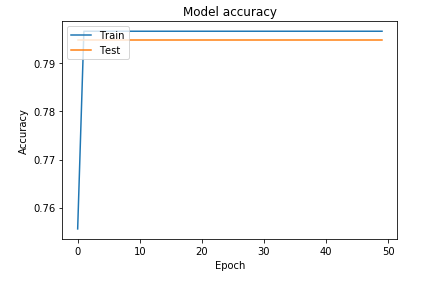
\includegraphics{https://uploaddeimagens.com.br/images/001/743/022/full/overfit.png?1543063949}

\emph{figura 6 - Resultado do overfitting}

A figura 7 mostra a rede neural utilizando 90 neurônios, nessa fase não
acontece o overfitting, pois o teste obtem melhores resultados que o
treino.
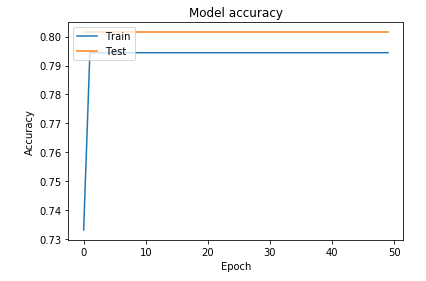
\includegraphics{https://uploaddeimagens.com.br/images/001/743/140/full/overfit2.png?1543073207}

\emph{figura 7 - Resultado do overfitting}

    \begin{Verbatim}[commandchars=\\\{\}]
{\color{incolor}In [{\color{incolor}12}]:} \PY{n}{model} \PY{o}{=} \PY{n}{Sequential}\PY{p}{(}\PY{p}{)}
         
         \PY{n}{model}\PY{o}{.}\PY{n}{add}\PY{p}{(}\PY{n}{Dense}\PY{p}{(}\PY{n}{units}\PY{o}{=}\PY{l+m+mi}{100}\PY{p}{,} \PY{n}{activation}\PY{o}{=}\PY{l+s+s1}{\PYZsq{}}\PY{l+s+s1}{relu}\PY{l+s+s1}{\PYZsq{}}\PY{p}{,} \PY{n}{input\PYZus{}dim}\PY{o}{=}\PY{n}{num\PYZus{}input}\PY{p}{)}\PY{p}{)}
         \PY{n}{model}\PY{o}{.}\PY{n}{add}\PY{p}{(}\PY{n}{Dense}\PY{p}{(}\PY{n}{units}\PY{o}{=}\PY{l+m+mi}{59}\PY{p}{,} \PY{n}{activation}\PY{o}{=}\PY{l+s+s1}{\PYZsq{}}\PY{l+s+s1}{relu}\PY{l+s+s1}{\PYZsq{}}\PY{p}{)}\PY{p}{)}
         \PY{n}{model}\PY{o}{.}\PY{n}{add}\PY{p}{(}\PY{n}{Dense}\PY{p}{(}\PY{l+m+mi}{1}\PY{p}{,} \PY{n}{activation}\PY{o}{=}\PY{l+s+s1}{\PYZsq{}}\PY{l+s+s1}{sigmoid}\PY{l+s+s1}{\PYZsq{}}\PY{p}{)}\PY{p}{)}
         
         \PY{n}{model}\PY{o}{.}\PY{n}{compile}\PY{p}{(}\PY{n}{loss}\PY{o}{=}\PY{l+s+s1}{\PYZsq{}}\PY{l+s+s1}{binary\PYZus{}crossentropy}\PY{l+s+s1}{\PYZsq{}}\PY{p}{,}
                       \PY{n}{optimizer}\PY{o}{=}\PY{l+s+s1}{\PYZsq{}}\PY{l+s+s1}{adam}\PY{l+s+s1}{\PYZsq{}}\PY{p}{,}
                       \PY{n}{metrics}\PY{o}{=}\PY{p}{[}\PY{l+s+s1}{\PYZsq{}}\PY{l+s+s1}{accuracy}\PY{l+s+s1}{\PYZsq{}}\PY{p}{]}\PY{p}{)}
         
         \PY{n}{history} \PY{o}{=} \PY{n}{model}\PY{o}{.}\PY{n}{fit}\PY{p}{(}\PY{n}{x\PYZus{}train}\PY{p}{,} \PY{n}{y\PYZus{}train}\PY{p}{,} \PY{n}{validation\PYZus{}split}\PY{o}{=}\PY{l+m+mf}{0.25}\PY{p}{,} \PY{n}{epochs}\PY{o}{=}\PY{l+m+mi}{50}\PY{p}{,} \PY{n}{batch\PYZus{}size}\PY{o}{=}\PY{l+m+mi}{16}\PY{p}{,} \PY{n}{verbose}\PY{o}{=}\PY{l+m+mi}{1}\PY{p}{)}
         
         \PY{n}{loss\PYZus{}and\PYZus{}metrics} \PY{o}{=} \PY{n}{model}\PY{o}{.}\PY{n}{evaluate}\PY{p}{(}\PY{n}{x\PYZus{}test}\PY{p}{,} \PY{n}{y\PYZus{}test}\PY{p}{,} \PY{n}{batch\PYZus{}size}\PY{o}{=}\PY{l+m+mi}{16}\PY{p}{)}
         \PY{n+nb}{print}\PY{p}{(}\PY{l+s+s2}{\PYZdq{}}\PY{l+s+se}{\PYZbs{}n}\PY{l+s+s2}{ Taxa de acerto: }\PY{l+s+si}{\PYZpc{}.2f}\PY{l+s+si}{\PYZpc{}\PYZpc{}}\PY{l+s+s2}{\PYZdq{}} \PY{o}{\PYZpc{}} \PY{p}{(}\PY{n}{loss\PYZus{}and\PYZus{}metrics}\PY{p}{[}\PY{l+m+mi}{1}\PY{p}{]}\PY{o}{*}\PY{l+m+mi}{100}\PY{p}{)}\PY{p}{)}
         
         \PY{c+c1}{\PYZsh{}optimizer : sgd }
         
         \PY{c+c1}{\PYZsh{} Plot training \PYZam{} validation accuracy values}
         \PY{n}{plt}\PY{o}{.}\PY{n}{plot}\PY{p}{(}\PY{n}{history}\PY{o}{.}\PY{n}{history}\PY{p}{[}\PY{l+s+s1}{\PYZsq{}}\PY{l+s+s1}{acc}\PY{l+s+s1}{\PYZsq{}}\PY{p}{]}\PY{p}{)}
         \PY{n}{plt}\PY{o}{.}\PY{n}{plot}\PY{p}{(}\PY{n}{history}\PY{o}{.}\PY{n}{history}\PY{p}{[}\PY{l+s+s1}{\PYZsq{}}\PY{l+s+s1}{val\PYZus{}acc}\PY{l+s+s1}{\PYZsq{}}\PY{p}{]}\PY{p}{)}
         \PY{n}{plt}\PY{o}{.}\PY{n}{title}\PY{p}{(}\PY{l+s+s1}{\PYZsq{}}\PY{l+s+s1}{Model accuracy}\PY{l+s+s1}{\PYZsq{}}\PY{p}{)}
         \PY{n}{plt}\PY{o}{.}\PY{n}{ylabel}\PY{p}{(}\PY{l+s+s1}{\PYZsq{}}\PY{l+s+s1}{Accuracy}\PY{l+s+s1}{\PYZsq{}}\PY{p}{)}
         \PY{n}{plt}\PY{o}{.}\PY{n}{xlabel}\PY{p}{(}\PY{l+s+s1}{\PYZsq{}}\PY{l+s+s1}{Epoch}\PY{l+s+s1}{\PYZsq{}}\PY{p}{)}
         \PY{n}{plt}\PY{o}{.}\PY{n}{legend}\PY{p}{(}\PY{p}{[}\PY{l+s+s1}{\PYZsq{}}\PY{l+s+s1}{Train}\PY{l+s+s1}{\PYZsq{}}\PY{p}{,} \PY{l+s+s1}{\PYZsq{}}\PY{l+s+s1}{Test}\PY{l+s+s1}{\PYZsq{}}\PY{p}{]}\PY{p}{,} \PY{n}{loc}\PY{o}{=}\PY{l+s+s1}{\PYZsq{}}\PY{l+s+s1}{upper left}\PY{l+s+s1}{\PYZsq{}}\PY{p}{)}
         \PY{n}{plt}\PY{o}{.}\PY{n}{show}\PY{p}{(}\PY{p}{)}
\end{Verbatim}


    \begin{Verbatim}[commandchars=\\\{\}]
Train on 20812 samples, validate on 6938 samples
Epoch 1/50
20812/20812 [==============================] - 12s 600us/step - loss: 5.5665 - acc: 0.6525 - val\_loss: 12.6978 - val\_acc: 0.2035
Epoch 2/50
20812/20812 [==============================] - 12s 580us/step - loss: 12.6922 - acc: 0.2039 - val\_loss: 12.6978 - val\_acc: 0.2035
Epoch 3/50
20812/20812 [==============================] - 12s 575us/step - loss: 12.6922 - acc: 0.2039 - val\_loss: 12.6978 - val\_acc: 0.2035
Epoch 4/50
20812/20812 [==============================] - 12s 558us/step - loss: 12.6922 - acc: 0.2039 - val\_loss: 12.6978 - val\_acc: 0.2035
Epoch 5/50
20812/20812 [==============================] - 12s 592us/step - loss: 12.6922 - acc: 0.2039 - val\_loss: 12.6978 - val\_acc: 0.2035
Epoch 6/50
20812/20812 [==============================] - 12s 582us/step - loss: 12.6922 - acc: 0.2039 - val\_loss: 12.6978 - val\_acc: 0.2035
Epoch 7/50
20812/20812 [==============================] - 14s 651us/step - loss: 12.6922 - acc: 0.2039 - val\_loss: 12.6978 - val\_acc: 0.2035
Epoch 8/50
20812/20812 [==============================] - 11s 546us/step - loss: 12.6922 - acc: 0.2039 - val\_loss: 12.6978 - val\_acc: 0.2035
Epoch 9/50
20812/20812 [==============================] - 13s 613us/step - loss: 12.6922 - acc: 0.2039 - val\_loss: 12.6978 - val\_acc: 0.2035
Epoch 10/50
20812/20812 [==============================] - 13s 605us/step - loss: 12.6922 - acc: 0.2039 - val\_loss: 12.6978 - val\_acc: 0.2035
Epoch 11/50
20812/20812 [==============================] - 13s 613us/step - loss: 12.6922 - acc: 0.2039 - val\_loss: 12.6978 - val\_acc: 0.2035
Epoch 12/50
20812/20812 [==============================] - 14s 664us/step - loss: 12.6922 - acc: 0.2039 - val\_loss: 12.6978 - val\_acc: 0.2035
Epoch 13/50
20812/20812 [==============================] - 14s 686us/step - loss: 12.6922 - acc: 0.2039 - val\_loss: 12.6978 - val\_acc: 0.2035
Epoch 14/50
20812/20812 [==============================] - 12s 600us/step - loss: 12.6922 - acc: 0.2039 - val\_loss: 12.6978 - val\_acc: 0.2035
Epoch 15/50
20812/20812 [==============================] - 12s 584us/step - loss: 12.6922 - acc: 0.2039 - val\_loss: 12.6978 - val\_acc: 0.2035
Epoch 16/50
20812/20812 [==============================] - 11s 537us/step - loss: 12.6922 - acc: 0.2039 - val\_loss: 12.6978 - val\_acc: 0.2035
Epoch 17/50
20812/20812 [==============================] - 12s 588us/step - loss: 12.6922 - acc: 0.2039 - val\_loss: 12.6978 - val\_acc: 0.2035
Epoch 18/50
20812/20812 [==============================] - 13s 604us/step - loss: 12.6922 - acc: 0.2039 - val\_loss: 12.6978 - val\_acc: 0.2035
Epoch 19/50
20812/20812 [==============================] - 13s 606us/step - loss: 12.6922 - acc: 0.2039 - val\_loss: 12.6978 - val\_acc: 0.2035
Epoch 20/50
20812/20812 [==============================] - 12s 591us/step - loss: 12.6922 - acc: 0.2039 - val\_loss: 12.6978 - val\_acc: 0.2035
Epoch 21/50
20812/20812 [==============================] - 11s 521us/step - loss: 12.6922 - acc: 0.2039 - val\_loss: 12.6978 - val\_acc: 0.2035
Epoch 22/50
20812/20812 [==============================] - 11s 530us/step - loss: 12.6922 - acc: 0.2039 - val\_loss: 12.6978 - val\_acc: 0.2035
Epoch 23/50
20812/20812 [==============================] - 11s 530us/step - loss: 12.6922 - acc: 0.2039 - val\_loss: 12.6978 - val\_acc: 0.2035
Epoch 24/50
20812/20812 [==============================] - 11s 546us/step - loss: 12.6922 - acc: 0.2039 - val\_loss: 12.6978 - val\_acc: 0.2035
Epoch 25/50
20812/20812 [==============================] - 11s 531us/step - loss: 12.6922 - acc: 0.2039 - val\_loss: 12.6978 - val\_acc: 0.2035
Epoch 26/50
20812/20812 [==============================] - 11s 510us/step - loss: 12.6922 - acc: 0.2039 - val\_loss: 12.6978 - val\_acc: 0.2035
Epoch 27/50
20812/20812 [==============================] - 11s 528us/step - loss: 12.6922 - acc: 0.2039 - val\_loss: 12.6978 - val\_acc: 0.2035
Epoch 28/50
20812/20812 [==============================] - 11s 510us/step - loss: 12.6922 - acc: 0.2039 - val\_loss: 12.6978 - val\_acc: 0.2035
Epoch 29/50
20812/20812 [==============================] - 11s 552us/step - loss: 12.6922 - acc: 0.2039 - val\_loss: 12.6978 - val\_acc: 0.2035
Epoch 30/50
20812/20812 [==============================] - 11s 507us/step - loss: 12.6922 - acc: 0.2039 - val\_loss: 12.6978 - val\_acc: 0.2035
Epoch 31/50
20812/20812 [==============================] - 11s 507us/step - loss: 12.6922 - acc: 0.2039 - val\_loss: 12.6978 - val\_acc: 0.2035
Epoch 32/50
20812/20812 [==============================] - 11s 513us/step - loss: 12.6922 - acc: 0.2039 - val\_loss: 12.6978 - val\_acc: 0.2035
Epoch 33/50
20812/20812 [==============================] - 13s 621us/step - loss: 12.6922 - acc: 0.2039 - val\_loss: 12.6978 - val\_acc: 0.2035
Epoch 34/50
20812/20812 [==============================] - 15s 708us/step - loss: 12.6922 - acc: 0.2039 - val\_loss: 12.6978 - val\_acc: 0.2035
Epoch 35/50
20812/20812 [==============================] - 12s 569us/step - loss: 12.6922 - acc: 0.2039 - val\_loss: 12.6978 - val\_acc: 0.2035
Epoch 36/50
20812/20812 [==============================] - 13s 621us/step - loss: 12.6922 - acc: 0.2039 - val\_loss: 12.6978 - val\_acc: 0.2035
Epoch 37/50
20812/20812 [==============================] - 12s 563us/step - loss: 12.6922 - acc: 0.2039 - val\_loss: 12.6978 - val\_acc: 0.2035
Epoch 38/50
20812/20812 [==============================] - 11s 531us/step - loss: 12.6922 - acc: 0.2039 - val\_loss: 12.6978 - val\_acc: 0.2035
Epoch 39/50
20812/20812 [==============================] - 11s 539us/step - loss: 12.6922 - acc: 0.2039 - val\_loss: 12.6978 - val\_acc: 0.2035
Epoch 40/50
20812/20812 [==============================] - 10s 496us/step - loss: 12.6922 - acc: 0.2039 - val\_loss: 12.6978 - val\_acc: 0.2035
Epoch 41/50
20812/20812 [==============================] - 10s 492us/step - loss: 12.6922 - acc: 0.2039 - val\_loss: 12.6978 - val\_acc: 0.2035
Epoch 42/50
20812/20812 [==============================] - 12s 562us/step - loss: 12.6922 - acc: 0.2039 - val\_loss: 12.6978 - val\_acc: 0.2035
Epoch 43/50
20812/20812 [==============================] - 14s 659us/step - loss: 12.6922 - acc: 0.2039 - val\_loss: 12.6978 - val\_acc: 0.2035
Epoch 44/50
20812/20812 [==============================] - 13s 605us/step - loss: 12.6922 - acc: 0.2039 - val\_loss: 12.6978 - val\_acc: 0.2035
Epoch 45/50
20812/20812 [==============================] - 13s 627us/step - loss: 12.6922 - acc: 0.2039 - val\_loss: 12.6978 - val\_acc: 0.2035
Epoch 46/50
20812/20812 [==============================] - 13s 637us/step - loss: 12.6922 - acc: 0.2039 - val\_loss: 12.6978 - val\_acc: 0.2035
Epoch 47/50
20812/20812 [==============================] - 12s 553us/step - loss: 12.6922 - acc: 0.2039 - val\_loss: 12.6978 - val\_acc: 0.2035
Epoch 48/50
20812/20812 [==============================] - 13s 606us/step - loss: 12.6922 - acc: 0.2039 - val\_loss: 12.6978 - val\_acc: 0.2035
Epoch 49/50
20812/20812 [==============================] - 12s 582us/step - loss: 12.6922 - acc: 0.2039 - val\_loss: 12.6978 - val\_acc: 0.2035
Epoch 50/50
20812/20812 [==============================] - 13s 621us/step - loss: 12.6922 - acc: 0.2039 - val\_loss: 12.6978 - val\_acc: 0.2035
11893/11893 [==============================] - 4s 335us/step

 Taxa de acerto: 20.38\%

    \end{Verbatim}

    \begin{center}
    \adjustimage{max size={0.9\linewidth}{0.9\paperheight}}{output_5_1.png}
    \end{center}
    { \hspace*{\fill} \\}
    
    \begin{center}
    \adjustimage{max size={0.9\linewidth}{0.9\paperheight}}{output_5_2.png}
    \end{center}
    { \hspace*{\fill} \\}
    
    Regularização

A regularização pode ajudar a reduzir o overfitting. Analisaremos os
efeitos de três técnicas de regularização no código, a técnica L1, L2 e
Dropout. A intenção da regularização é fazer com que a rede prefira
aprender pesos pequenos. Os pesos grandes só são permitidos se
melhorarem bastante a primeira parte da função de custo, ou seja, ela
tenta encontrar pequenos pesos e minimizar a função de custo original.

Tanto na técnica L1 quanto na L2 o resultado é a diminuição dos valores
dos pesos, mas a maneira como os pesos diminuem é diferente. Quando um
peso específico tem uma grande magnitude, a regularização L1 reduz o
peso muito menos do que a Regularização L2, mas, quando
\textbar{}w\textbar{} é pequeno, a regularização L1 reduz o peso muito
mais do que a regularização L2, assim a regularização L1 tende a
concentrar o peso da rede em um número relativamente pequeno de conexões
de alta importância, enquanto os outros pesos são direcionados para
zero.

Configurações utilizadas no modelo de regularização L1:

    \begin{Verbatim}[commandchars=\\\{\}]
{\color{incolor}In [{\color{incolor} }]:} \PY{n}{model} \PY{o}{=} \PY{n}{Sequential}\PY{p}{(}\PY{p}{)}
        
        \PY{n}{model}\PY{o}{.}\PY{n}{add}\PY{p}{(}\PY{n}{Dense}\PY{p}{(}\PY{n}{units}\PY{o}{=}\PY{l+m+mi}{100}\PY{p}{,} \PY{n}{activation}\PY{o}{=}\PY{l+s+s1}{\PYZsq{}}\PY{l+s+s1}{relu}\PY{l+s+s1}{\PYZsq{}}\PY{p}{,} \PY{n}{input\PYZus{}dim}\PY{o}{=}\PY{n}{num\PYZus{}input}\PY{p}{,} \PY{n}{activity\PYZus{}regularizer}\PY{o}{=}\PY{n}{regularizers}\PY{o}{.}\PY{n}{l1}\PY{p}{(}\PY{l+m+mf}{0.01}\PY{p}{)}\PY{p}{)}\PY{p}{)}
        \PY{n}{model}\PY{o}{.}\PY{n}{add}\PY{p}{(}\PY{n}{Dense}\PY{p}{(}\PY{n}{units}\PY{o}{=}\PY{l+m+mi}{59}\PY{p}{,} \PY{n}{activation}\PY{o}{=}\PY{l+s+s1}{\PYZsq{}}\PY{l+s+s1}{relu}\PY{l+s+s1}{\PYZsq{}}\PY{p}{,} \PY{n}{activity\PYZus{}regularizer}\PY{o}{=}\PY{n}{regularizers}\PY{o}{.}\PY{n}{l1}\PY{p}{(}\PY{l+m+mf}{0.01}\PY{p}{)}\PY{p}{)}\PY{p}{)}
        \PY{n}{model}\PY{o}{.}\PY{n}{add}\PY{p}{(}\PY{n}{Dense}\PY{p}{(}\PY{l+m+mi}{1}\PY{p}{,} \PY{n}{activation}\PY{o}{=}\PY{l+s+s1}{\PYZsq{}}\PY{l+s+s1}{sigmoid}\PY{l+s+s1}{\PYZsq{}}\PY{p}{)}\PY{p}{)}
        
        \PY{n}{model}\PY{o}{.}\PY{n}{compile}\PY{p}{(}\PY{n}{loss}\PY{o}{=}\PY{l+s+s1}{\PYZsq{}}\PY{l+s+s1}{binary\PYZus{}crossentropy}\PY{l+s+s1}{\PYZsq{}}\PY{p}{,} \PY{n}{optimizer}\PY{o}{=}\PY{l+s+s1}{\PYZsq{}}\PY{l+s+s1}{adam}\PY{l+s+s1}{\PYZsq{}}\PY{p}{,} \PY{n}{metrics}\PY{o}{=}\PY{p}{[}\PY{l+s+s1}{\PYZsq{}}\PY{l+s+s1}{accuracy}\PY{l+s+s1}{\PYZsq{}}\PY{p}{]}\PY{p}{)}
        
        \PY{n}{history} \PY{o}{=} \PY{n}{model}\PY{o}{.}\PY{n}{fit}\PY{p}{(}\PY{n}{x\PYZus{}train}\PY{p}{,} \PY{n}{y\PYZus{}train}\PY{p}{,} \PY{n}{validation\PYZus{}split}\PY{o}{=}\PY{l+m+mf}{0.25}\PY{p}{,} \PY{n}{epochs}\PY{o}{=}\PY{l+m+mi}{50}\PY{p}{,} \PY{n}{batch\PYZus{}size}\PY{o}{=}\PY{l+m+mi}{16}\PY{p}{,} \PY{n}{verbose}\PY{o}{=}\PY{l+m+mi}{1}\PY{p}{)}
        
        \PY{n}{loss\PYZus{}and\PYZus{}metrics} \PY{o}{=} \PY{n}{model}\PY{o}{.}\PY{n}{evaluate}\PY{p}{(}\PY{n}{x\PYZus{}test}\PY{p}{,} \PY{n}{y\PYZus{}test}\PY{p}{,} \PY{n}{batch\PYZus{}size}\PY{o}{=}\PY{l+m+mi}{16}\PY{p}{)}
\end{Verbatim}


    Com essas configurações no L1 foi obtido uma taxa de acerto de 79,63\%.
A figura 8 demostra o histórico da acurácia para o L1 com valor de 0.1.
\includegraphics{https://uploaddeimagens.com.br/images/001/744/765/full/l1-0_01.png?1543200998}

\emph{figura 8 - Histórico de acurácia para L1 = 0.1}

A figura 9 demostra o histórico da acurácia para o L1 com valor de de
0.01 nesse caso o resultado do teste apresentou ser pior do que o
utilizado com 0.1, pois a taxa de acerto obtida foi de 79,60\%.

\includegraphics{https://uploaddeimagens.com.br/images/001/744/780/full/l1-0_01.png?1543201813}

\emph{figura 9 - Histórico de acurácia para L1 = 0.01}

    Configurações utilizadas no modelo de regularização L2:

    \begin{Verbatim}[commandchars=\\\{\}]
{\color{incolor}In [{\color{incolor} }]:} \PY{n}{model} \PY{o}{=} \PY{n}{Sequential}\PY{p}{(}\PY{p}{)}
        
        \PY{n}{model}\PY{o}{.}\PY{n}{add}\PY{p}{(}\PY{n}{Dense}\PY{p}{(}\PY{n}{units}\PY{o}{=}\PY{l+m+mi}{100}\PY{p}{,} \PY{n}{activation}\PY{o}{=}\PY{l+s+s1}{\PYZsq{}}\PY{l+s+s1}{relu}\PY{l+s+s1}{\PYZsq{}}\PY{p}{,} \PY{n}{input\PYZus{}dim}\PY{o}{=}\PY{n}{num\PYZus{}input}\PY{p}{,} \PY{n}{kernel\PYZus{}regularizer}\PY{o}{=}\PY{n}{regularizers}\PY{o}{.}\PY{n}{l2}\PY{p}{(}\PY{l+m+mf}{0.01}\PY{p}{)}\PY{p}{)}\PY{p}{)}
        \PY{n}{model}\PY{o}{.}\PY{n}{add}\PY{p}{(}\PY{n}{Dense}\PY{p}{(}\PY{n}{units}\PY{o}{=}\PY{l+m+mi}{59}\PY{p}{,} \PY{n}{activation}\PY{o}{=}\PY{l+s+s1}{\PYZsq{}}\PY{l+s+s1}{relu}\PY{l+s+s1}{\PYZsq{}}\PY{p}{,} \PY{n}{kernel\PYZus{}regularizer}\PY{o}{=}\PY{n}{regularizers}\PY{o}{.}\PY{n}{l2}\PY{p}{(}\PY{l+m+mf}{0.01}\PY{p}{)}\PY{p}{)}\PY{p}{)}
        \PY{n}{model}\PY{o}{.}\PY{n}{add}\PY{p}{(}\PY{n}{Dense}\PY{p}{(}\PY{l+m+mi}{1}\PY{p}{,} \PY{n}{activation}\PY{o}{=}\PY{l+s+s1}{\PYZsq{}}\PY{l+s+s1}{sigmoid}\PY{l+s+s1}{\PYZsq{}}\PY{p}{)}\PY{p}{)}
        
        \PY{n}{model}\PY{o}{.}\PY{n}{compile}\PY{p}{(}\PY{n}{loss}\PY{o}{=}\PY{l+s+s1}{\PYZsq{}}\PY{l+s+s1}{binary\PYZus{}crossentropy}\PY{l+s+s1}{\PYZsq{}}\PY{p}{,} \PY{n}{optimizer}\PY{o}{=}\PY{l+s+s1}{\PYZsq{}}\PY{l+s+s1}{adam}\PY{l+s+s1}{\PYZsq{}}\PY{p}{,} \PY{n}{metrics}\PY{o}{=}\PY{p}{[}\PY{l+s+s1}{\PYZsq{}}\PY{l+s+s1}{accuracy}\PY{l+s+s1}{\PYZsq{}}\PY{p}{]}\PY{p}{)}
        
        \PY{n}{history} \PY{o}{=} \PY{n}{model}\PY{o}{.}\PY{n}{fit}\PY{p}{(}\PY{n}{x\PYZus{}train}\PY{p}{,} \PY{n}{y\PYZus{}train}\PY{p}{,} \PY{n}{validation\PYZus{}split}\PY{o}{=}\PY{l+m+mf}{0.25}\PY{p}{,} \PY{n}{epochs}\PY{o}{=}\PY{l+m+mi}{50}\PY{p}{,} \PY{n}{batch\PYZus{}size}\PY{o}{=}\PY{l+m+mi}{16}\PY{p}{,} \PY{n}{verbose}\PY{o}{=}\PY{l+m+mi}{1}\PY{p}{)}
        
        \PY{n}{loss\PYZus{}and\PYZus{}metrics} \PY{o}{=} \PY{n}{model}\PY{o}{.}\PY{n}{evaluate}\PY{p}{(}\PY{n}{x\PYZus{}test}\PY{p}{,} \PY{n}{y\PYZus{}test}\PY{p}{,} \PY{n}{batch\PYZus{}size}\PY{o}{=}\PY{l+m+mi}{16}\PY{p}{)}
\end{Verbatim}


    Com essas configurações no L2 foi obtido uma taxa de acerto de 79,62\%.
A figura 10 demostra o histórico da acurácia para o L1 com valor de
0.01, a média da taxa de acerto de treino é de 79,61\% e de teste é de
79,65\%.
\includegraphics{https://uploaddeimagens.com.br/images/001/744/708/full/l2-0_01.png?1543197697}

\emph{figura 10 - Histórico de acurácia para L2 = 0.01}

A figura 11 demostra o histórico da acurácia para o L2 com valor de de
0.1, nesse caso o resultado do teste apresentou ser praticamente o mesmo
que o anterior.

\includegraphics{https://uploaddeimagens.com.br/images/001/744/722/full/l2-0_1.png?1543199138}

\emph{figura 11 - Histórico de acurácia para L2 = 0.1}

    O Dropout é uma técnica diferente da L1 e L2, ele não depende da
modificação da função de custo, ele modifica a própria rede. O Dropout
elimina aleatoriamente (e temporariamente) alguns dos neurônios ocultos
na rede, mas deixa os neurônios de entrada e saída intocados.

Configurações utilizadas no Dropout:

    \begin{Verbatim}[commandchars=\\\{\}]
{\color{incolor}In [{\color{incolor} }]:} \PY{n}{model} \PY{o}{=} \PY{n}{Sequential}\PY{p}{(}\PY{p}{)}
        
        \PY{n}{model}\PY{o}{.}\PY{n}{add}\PY{p}{(}\PY{n}{Dense}\PY{p}{(}\PY{n}{units}\PY{o}{=}\PY{l+m+mi}{100}\PY{p}{,} \PY{n}{activation}\PY{o}{=}\PY{l+s+s1}{\PYZsq{}}\PY{l+s+s1}{relu}\PY{l+s+s1}{\PYZsq{}}\PY{p}{,} \PY{n}{input\PYZus{}dim}\PY{o}{=}\PY{n}{num\PYZus{}input}\PY{p}{)}
        \PY{n}{model}\PY{o}{.}\PY{n}{add}\PY{p}{(}\PY{n}{Dropout}\PY{p}{(}\PY{l+m+mf}{0.5}\PY{p}{)}\PY{p}{)}
        \PY{n}{model}\PY{o}{.}\PY{n}{add}\PY{p}{(}\PY{n}{Dense}\PY{p}{(}\PY{n}{units}\PY{o}{=}\PY{l+m+mi}{59}\PY{p}{,} \PY{n}{activation}\PY{o}{=}\PY{l+s+s1}{\PYZsq{}}\PY{l+s+s1}{relu}\PY{l+s+s1}{\PYZsq{}}\PY{p}{)}\PY{p}{)}
        \PY{n}{model}\PY{o}{.}\PY{n}{add}\PY{p}{(}\PY{n}{Dropout}\PY{p}{(}\PY{l+m+mf}{0.5}\PY{p}{)}\PY{p}{)}
        \PY{n}{model}\PY{o}{.}\PY{n}{add}\PY{p}{(}\PY{n}{Dense}\PY{p}{(}\PY{l+m+mi}{1}\PY{p}{,} \PY{n}{activation}\PY{o}{=}\PY{l+s+s1}{\PYZsq{}}\PY{l+s+s1}{sigmoid}\PY{l+s+s1}{\PYZsq{}}\PY{p}{)}\PY{p}{)}
        
        \PY{n}{model}\PY{o}{.}\PY{n}{compile}\PY{p}{(}\PY{n}{loss}\PY{o}{=}\PY{l+s+s1}{\PYZsq{}}\PY{l+s+s1}{binary\PYZus{}crossentropy}\PY{l+s+s1}{\PYZsq{}}\PY{p}{,} \PY{n}{optimizer}\PY{o}{=}\PY{l+s+s1}{\PYZsq{}}\PY{l+s+s1}{adam}\PY{l+s+s1}{\PYZsq{}}\PY{p}{,} \PY{n}{metrics}\PY{o}{=}\PY{p}{[}\PY{l+s+s1}{\PYZsq{}}\PY{l+s+s1}{accuracy}\PY{l+s+s1}{\PYZsq{}}\PY{p}{]}\PY{p}{)}
        
        \PY{n}{history} \PY{o}{=} \PY{n}{model}\PY{o}{.}\PY{n}{fit}\PY{p}{(}\PY{n}{x\PYZus{}train}\PY{p}{,} \PY{n}{y\PYZus{}train}\PY{p}{,} \PY{n}{validation\PYZus{}split}\PY{o}{=}\PY{l+m+mf}{0.25}\PY{p}{,} \PY{n}{epochs}\PY{o}{=}\PY{l+m+mi}{50}\PY{p}{,} \PY{n}{batch\PYZus{}size}\PY{o}{=}\PY{l+m+mi}{16}\PY{p}{,} \PY{n}{verbose}\PY{o}{=}\PY{l+m+mi}{1}\PY{p}{)}
        
        \PY{n}{loss\PYZus{}and\PYZus{}metrics} \PY{o}{=} \PY{n}{model}\PY{o}{.}\PY{n}{evaluate}\PY{p}{(}\PY{n}{x\PYZus{}test}\PY{p}{,} \PY{n}{y\PYZus{}test}\PY{p}{,} \PY{n}{batch\PYZus{}size}\PY{o}{=}\PY{l+m+mi}{16}\PY{p}{)}
\end{Verbatim}


    Com o Dropout de 0.5 foi obtido uma taxa de acerto de 79,62\%, a figura
12 mostra o histórico da acurácia na fase de treino e teste.

\includegraphics{https://uploaddeimagens.com.br/images/001/744/803/full/drop-0_5.png?1543204505}

\emph{figura 12 - Histórico de acurácia para Dropout = 0.5}

Com o Dropout de 0.3 foi obtido uma taxa de acerto de 79,62\%, a figura
13 mostra o histórico da acurácia na fase de treino e teste.

\includegraphics{https://uploaddeimagens.com.br/images/001/744/821/full/drop-0_3.png?1543206419}

\emph{figura 13 - Histórico de acurácia para Dropout = 0.3}

Com o Dropout de 0.7 foi obtido uma taxa de acerto de 79,62\%, a figura
14 mostra o histórico da acurácia na fase de treino e teste.

\includegraphics{https://uploaddeimagens.com.br/images/001/744/819/full/drop-0_7.png?1543206380}

\emph{figura 14 - Histórico de acurácia para Dropout = 0.7}

    Hiperparâmetros

Inicialmente será decidido o número de neuronios utilizados na segunda e
terceira camada, como mostra o código a seguir:

    \begin{Verbatim}[commandchars=\\\{\}]
{\color{incolor}In [{\color{incolor} }]:} \PY{n}{model} \PY{o}{=} \PY{n}{Sequential}\PY{p}{(}\PY{p}{)}
        
        \PY{n}{model}\PY{o}{.}\PY{n}{add}\PY{p}{(}\PY{n}{Dense}\PY{p}{(}\PY{n}{units}\PY{o}{=}\PY{l+m+mi}{80}\PY{p}{,} \PY{n}{activation}\PY{o}{=}\PY{l+s+s1}{\PYZsq{}}\PY{l+s+s1}{relu}\PY{l+s+s1}{\PYZsq{}}\PY{p}{,} \PY{n}{input\PYZus{}dim}\PY{o}{=}\PY{n}{num\PYZus{}input}\PY{p}{)}\PY{p}{)}
        \PY{n}{model}\PY{o}{.}\PY{n}{add}\PY{p}{(}\PY{n}{Dense}\PY{p}{(}\PY{n}{units}\PY{o}{=}\PY{l+m+mi}{20}\PY{p}{,} \PY{n}{activation}\PY{o}{=}\PY{l+s+s1}{\PYZsq{}}\PY{l+s+s1}{relu}\PY{l+s+s1}{\PYZsq{}}\PY{p}{)}\PY{p}{)}
        \PY{n}{model}\PY{o}{.}\PY{n}{add}\PY{p}{(}\PY{n}{Dense}\PY{p}{(}\PY{l+m+mi}{1}\PY{p}{,} \PY{n}{activation}\PY{o}{=}\PY{l+s+s1}{\PYZsq{}}\PY{l+s+s1}{sigmoid}\PY{l+s+s1}{\PYZsq{}}\PY{p}{)}\PY{p}{)}
        
        \PY{n}{model}\PY{o}{.}\PY{n}{compile}\PY{p}{(}\PY{n}{loss}\PY{o}{=}\PY{l+s+s1}{\PYZsq{}}\PY{l+s+s1}{binary\PYZus{}crossentropy}\PY{l+s+s1}{\PYZsq{}}\PY{p}{,} \PY{n}{optimizer}\PY{o}{=}\PY{l+s+s1}{\PYZsq{}}\PY{l+s+s1}{adam}\PY{l+s+s1}{\PYZsq{}}\PY{p}{,} \PY{n}{metrics}\PY{o}{=}\PY{p}{[}\PY{l+s+s1}{\PYZsq{}}\PY{l+s+s1}{accuracy}\PY{l+s+s1}{\PYZsq{}}\PY{p}{]}\PY{p}{)}
        
        \PY{n}{history} \PY{o}{=} \PY{n}{model}\PY{o}{.}\PY{n}{fit}\PY{p}{(}\PY{n}{x\PYZus{}train}\PY{p}{,} \PY{n}{y\PYZus{}train}\PY{p}{,} \PY{n}{validation\PYZus{}split}\PY{o}{=}\PY{l+m+mf}{0.25}\PY{p}{,} \PY{n}{epochs}\PY{o}{=}\PY{l+m+mi}{20}\PY{p}{,} \PY{n}{batch\PYZus{}size}\PY{o}{=}\PY{l+m+mi}{16}\PY{p}{,} \PY{n}{verbose}\PY{o}{=}\PY{l+m+mi}{1}\PY{p}{)}
\end{Verbatim}


    A figura 15 mostra o histórico da acurácia obtido, utilizando 20
neurônios na segunda camada oculta. A taxa de acerto foi de 79,7\%.

\includegraphics{https://uploaddeimagens.com.br/images/001/744/819/full/drop-0_7.png?1543206380}

\emph{figura 15 - Histórico de acurácia para 2² camada oculta = 20}

    \begin{Verbatim}[commandchars=\\\{\}]
{\color{incolor}In [{\color{incolor}31}]:} \PY{n}{model} \PY{o}{=} \PY{n}{Sequential}\PY{p}{(}\PY{p}{)}
         
         \PY{n}{model}\PY{o}{.}\PY{n}{add}\PY{p}{(}\PY{n}{Dense}\PY{p}{(}\PY{n}{units}\PY{o}{=}\PY{l+m+mi}{80}\PY{p}{,} \PY{n}{activation}\PY{o}{=}\PY{l+s+s1}{\PYZsq{}}\PY{l+s+s1}{relu}\PY{l+s+s1}{\PYZsq{}}\PY{p}{,} \PY{n}{input\PYZus{}dim}\PY{o}{=}\PY{n}{num\PYZus{}input}\PY{p}{)}\PY{p}{)}
         \PY{n}{model}\PY{o}{.}\PY{n}{add}\PY{p}{(}\PY{n}{Dense}\PY{p}{(}\PY{n}{units}\PY{o}{=}\PY{l+m+mi}{120}\PY{p}{,} \PY{n}{activation}\PY{o}{=}\PY{l+s+s1}{\PYZsq{}}\PY{l+s+s1}{relu}\PY{l+s+s1}{\PYZsq{}}\PY{p}{)}\PY{p}{)}
         \PY{n}{model}\PY{o}{.}\PY{n}{add}\PY{p}{(}\PY{n}{Dense}\PY{p}{(}\PY{l+m+mi}{1}\PY{p}{,} \PY{n}{activation}\PY{o}{=}\PY{l+s+s1}{\PYZsq{}}\PY{l+s+s1}{sigmoid}\PY{l+s+s1}{\PYZsq{}}\PY{p}{)}\PY{p}{)}
         
         \PY{n}{model}\PY{o}{.}\PY{n}{compile}\PY{p}{(}\PY{n}{loss}\PY{o}{=}\PY{l+s+s1}{\PYZsq{}}\PY{l+s+s1}{binary\PYZus{}crossentropy}\PY{l+s+s1}{\PYZsq{}}\PY{p}{,} \PY{n}{optimizer}\PY{o}{=}\PY{l+s+s1}{\PYZsq{}}\PY{l+s+s1}{adam}\PY{l+s+s1}{\PYZsq{}}\PY{p}{,} \PY{n}{metrics}\PY{o}{=}\PY{p}{[}\PY{l+s+s1}{\PYZsq{}}\PY{l+s+s1}{accuracy}\PY{l+s+s1}{\PYZsq{}}\PY{p}{]}\PY{p}{)}
         
         \PY{n}{history} \PY{o}{=} \PY{n}{model}\PY{o}{.}\PY{n}{fit}\PY{p}{(}\PY{n}{x\PYZus{}train}\PY{p}{,} \PY{n}{y\PYZus{}train}\PY{p}{,} \PY{n}{validation\PYZus{}split}\PY{o}{=}\PY{l+m+mf}{0.25}\PY{p}{,} \PY{n}{epochs}\PY{o}{=}\PY{l+m+mi}{20}\PY{p}{,} \PY{n}{batch\PYZus{}size}\PY{o}{=}\PY{l+m+mi}{16}\PY{p}{,} \PY{n}{verbose}\PY{o}{=}\PY{l+m+mi}{1}\PY{p}{)}
         
         \PY{n}{loss\PYZus{}and\PYZus{}metrics} \PY{o}{=} \PY{n}{model}\PY{o}{.}\PY{n}{evaluate}\PY{p}{(}\PY{n}{x\PYZus{}test}\PY{p}{,} \PY{n}{y\PYZus{}test}\PY{p}{,} \PY{n}{batch\PYZus{}size}\PY{o}{=}\PY{l+m+mi}{16}\PY{p}{)}
         \PY{n+nb}{print}\PY{p}{(}\PY{l+s+s2}{\PYZdq{}}\PY{l+s+se}{\PYZbs{}n}\PY{l+s+s2}{ Taxa de acerto: }\PY{l+s+si}{\PYZpc{}.2f}\PY{l+s+si}{\PYZpc{}\PYZpc{}}\PY{l+s+s2}{\PYZdq{}} \PY{o}{\PYZpc{}} \PY{p}{(}\PY{n}{loss\PYZus{}and\PYZus{}metrics}\PY{p}{[}\PY{l+m+mi}{1}\PY{p}{]}\PY{o}{*}\PY{l+m+mi}{100}\PY{p}{)}\PY{p}{)}
         \PY{c+c1}{\PYZsh{}optimizer : sgd }
         
         \PY{c+c1}{\PYZsh{} Plot training \PYZam{} validation accuracy values}
         \PY{n}{plt}\PY{o}{.}\PY{n}{plot}\PY{p}{(}\PY{n}{history}\PY{o}{.}\PY{n}{history}\PY{p}{[}\PY{l+s+s1}{\PYZsq{}}\PY{l+s+s1}{acc}\PY{l+s+s1}{\PYZsq{}}\PY{p}{]}\PY{p}{)}
         \PY{n}{plt}\PY{o}{.}\PY{n}{plot}\PY{p}{(}\PY{n}{history}\PY{o}{.}\PY{n}{history}\PY{p}{[}\PY{l+s+s1}{\PYZsq{}}\PY{l+s+s1}{val\PYZus{}acc}\PY{l+s+s1}{\PYZsq{}}\PY{p}{]}\PY{p}{)}
         \PY{n}{plt}\PY{o}{.}\PY{n}{title}\PY{p}{(}\PY{l+s+s1}{\PYZsq{}}\PY{l+s+s1}{Model accuracy}\PY{l+s+s1}{\PYZsq{}}\PY{p}{)}
         \PY{n}{plt}\PY{o}{.}\PY{n}{ylabel}\PY{p}{(}\PY{l+s+s1}{\PYZsq{}}\PY{l+s+s1}{Accuracy}\PY{l+s+s1}{\PYZsq{}}\PY{p}{)}
         \PY{n}{plt}\PY{o}{.}\PY{n}{xlabel}\PY{p}{(}\PY{l+s+s1}{\PYZsq{}}\PY{l+s+s1}{Epoch}\PY{l+s+s1}{\PYZsq{}}\PY{p}{)}
         \PY{n}{plt}\PY{o}{.}\PY{n}{legend}\PY{p}{(}\PY{p}{[}\PY{l+s+s1}{\PYZsq{}}\PY{l+s+s1}{Train}\PY{l+s+s1}{\PYZsq{}}\PY{p}{,} \PY{l+s+s1}{\PYZsq{}}\PY{l+s+s1}{Test}\PY{l+s+s1}{\PYZsq{}}\PY{p}{]}\PY{p}{,} \PY{n}{loc}\PY{o}{=}\PY{l+s+s1}{\PYZsq{}}\PY{l+s+s1}{upper left}\PY{l+s+s1}{\PYZsq{}}\PY{p}{)}
         \PY{n}{plt}\PY{o}{.}\PY{n}{show}\PY{p}{(}\PY{p}{)}
\end{Verbatim}


    \begin{Verbatim}[commandchars=\\\{\}]
Train on 20812 samples, validate on 6938 samples
Epoch 1/20
20812/20812 [==============================] - 14s 695us/step - loss: 4.0393 - acc: 0.7487 - val\_loss: 3.2547 - val\_acc: 0.7981
Epoch 2/20
20812/20812 [==============================] - 13s 615us/step - loss: 3.2946 - acc: 0.7956 - val\_loss: 3.2547 - val\_acc: 0.7981
Epoch 3/20
20812/20812 [==============================] - 12s 572us/step - loss: 3.2946 - acc: 0.7956 - val\_loss: 3.2547 - val\_acc: 0.7981
Epoch 4/20
20812/20812 [==============================] - 12s 555us/step - loss: 3.2946 - acc: 0.7956 - val\_loss: 3.2547 - val\_acc: 0.7981
Epoch 5/20
20812/20812 [==============================] - 12s 560us/step - loss: 3.2946 - acc: 0.7956 - val\_loss: 3.2547 - val\_acc: 0.7981
Epoch 6/20
20812/20812 [==============================] - 11s 541us/step - loss: 3.2946 - acc: 0.7956 - val\_loss: 3.2547 - val\_acc: 0.7981
Epoch 7/20
20812/20812 [==============================] - 12s 598us/step - loss: 3.2946 - acc: 0.7956 - val\_loss: 3.2547 - val\_acc: 0.7981
Epoch 8/20
20812/20812 [==============================] - 15s 703us/step - loss: 3.2946 - acc: 0.7956 - val\_loss: 3.2547 - val\_acc: 0.7981
Epoch 9/20
20812/20812 [==============================] - 14s 654us/step - loss: 3.2946 - acc: 0.7956 - val\_loss: 3.2547 - val\_acc: 0.7981
Epoch 10/20
20812/20812 [==============================] - 12s 600us/step - loss: 3.2946 - acc: 0.7956 - val\_loss: 3.2547 - val\_acc: 0.7981
Epoch 11/20
20812/20812 [==============================] - 13s 613us/step - loss: 3.2946 - acc: 0.7956 - val\_loss: 3.2547 - val\_acc: 0.7981
Epoch 12/20
20812/20812 [==============================] - 13s 621us/step - loss: 3.2946 - acc: 0.7956 - val\_loss: 3.2547 - val\_acc: 0.7981
Epoch 13/20
20812/20812 [==============================] - 14s 692us/step - loss: 3.2946 - acc: 0.7956 - val\_loss: 3.2547 - val\_acc: 0.7981
Epoch 14/20
20812/20812 [==============================] - 13s 638us/step - loss: 3.2946 - acc: 0.7956 - val\_loss: 3.2547 - val\_acc: 0.7981
Epoch 15/20
20812/20812 [==============================] - 12s 572us/step - loss: 3.2946 - acc: 0.7956 - val\_loss: 3.2547 - val\_acc: 0.7981
Epoch 16/20
20812/20812 [==============================] - 13s 622us/step - loss: 3.2946 - acc: 0.7956 - val\_loss: 3.2547 - val\_acc: 0.7981
Epoch 17/20
20812/20812 [==============================] - 14s 667us/step - loss: 3.2946 - acc: 0.7956 - val\_loss: 3.2547 - val\_acc: 0.7981
Epoch 18/20
20812/20812 [==============================] - 14s 669us/step - loss: 3.2946 - acc: 0.7956 - val\_loss: 3.2547 - val\_acc: 0.7981
Epoch 19/20
20812/20812 [==============================] - 12s 573us/step - loss: 3.2946 - acc: 0.7956 - val\_loss: 3.2547 - val\_acc: 0.7981
Epoch 20/20
20812/20812 [==============================] - 13s 637us/step - loss: 3.2946 - acc: 0.7956 - val\_loss: 3.2547 - val\_acc: 0.7981
11893/11893 [==============================] - 3s 242us/step

 Taxa de acerto: 79.62\%

    \end{Verbatim}

    \begin{center}
    \adjustimage{max size={0.9\linewidth}{0.9\paperheight}}{output_18_1.png}
    \end{center}
    { \hspace*{\fill} \\}
    

    % Add a bibliography block to the postdoc
    
    
    
    \end{document}
